%mainfile: ../../master.tex
\subsection{Structure}\label{sub:structure}

\cref{fig:structure} describe what classes are associated to what classes. This will be useful for the designers and system when designing and reasoning about the knowledge base \cref{sub:KB}.

\begin{figure}
  \label{fig:structure}
  \centering
  \begin{adjustbox}{max width=\textwidth}
    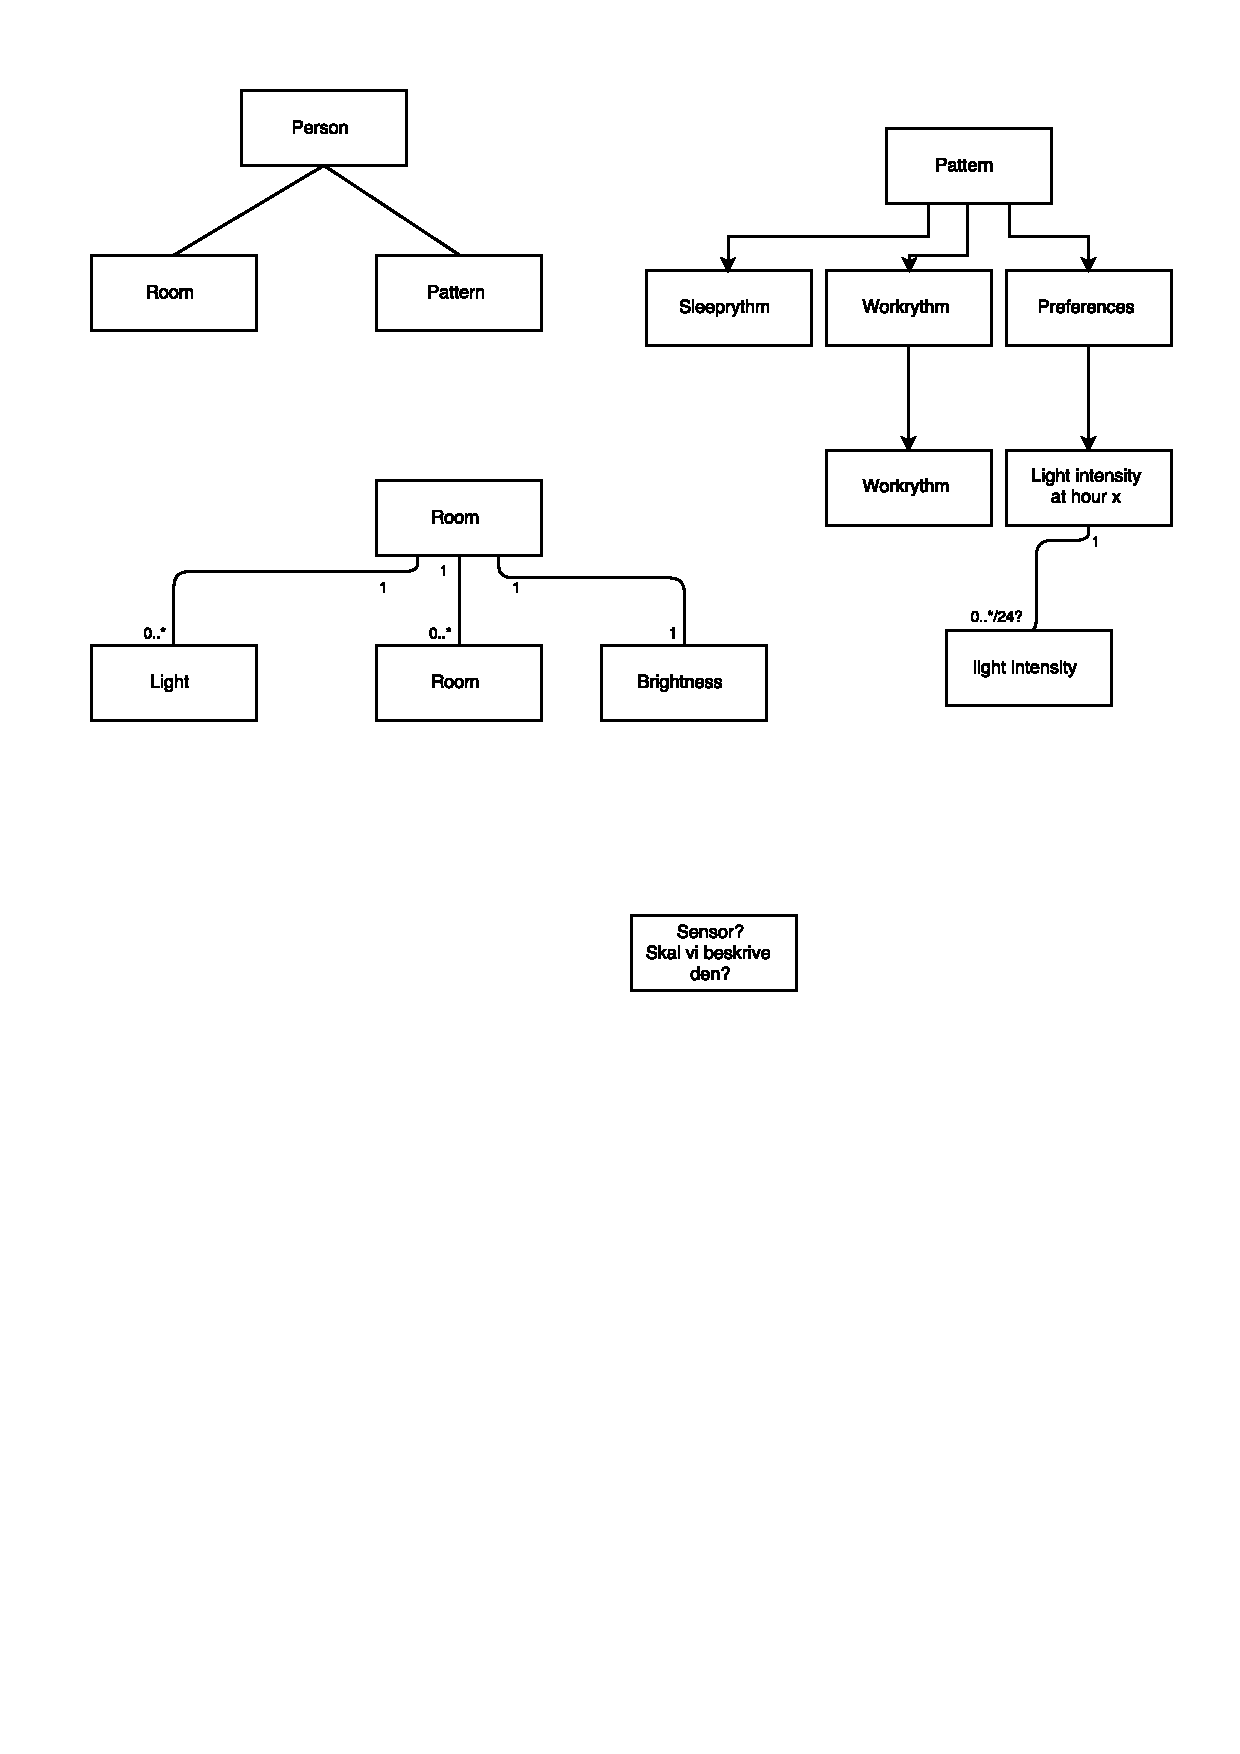
\includegraphics{Structure.pdf}
  \end{adjustbox}
  \caption{Structure of the problem domain}
\end{figure}
